\documentclass[11pt]{article} %This sets the font size and the document class of your report. In this case we use 'article' as that is ideal for shorter reports.
\usepackage{amssymb}
\usepackage{amsmath}
% LaTeX can be enhanced by the use of packages. These packages can do many things, a few of the most common and useful are used here. They are declared before the document proper, in what is known as the 'preamble'. Packages need to be installed when a .tex file compiles into a .pdf, but should do so automatically.
\usepackage[skip=0.5ex]{subcaption}
\usepackage[top=2.54cm, bottom=2.54cm, left=2.75cm, right=2.75cm]{geometry} %This sets the margins of the report.

\usepackage{graphicx} % A package allowing insertion of images into the text.
\usepackage{caption}

% Choose your citations style by commenting out one of the following groups. If you decide to change style, you should also delete the .bbl file that you will find in the same folder as your .tex and .pdf files.

% IEEE style citation:
\usepackage[style=ieee]{biblatex}
\addbibresource{sem_2_report.bib}

%% Author-date style citation:
%\usepackage[round]{natbib} % A package that creates references in the author-date style, with round brackets
%\renewcommand{\cite}{\citep} % For use with natbib only: comment out for the cite package.
%\bibliographystyle{plainnat} % Author-date referencing (use in conjunction with the natbib package)
\usepackage{color} % Allows the colour of the font to be changed by using the '\color' command: This is just to support the blue comments in this template...use standard (black) text in your report.
\usepackage{float}
\usepackage{subdepth}
\usepackage{mathtools}
\usepackage{tabularx}
\usepackage{makecell}
\linespread{1} % Sets the spacing between lines of text.
\setlength{\parindent}{0cm}  % Suppresses indentation of text at the start of a paragraph
\pagenumbering{arabic} % sets the style of page numbering for the report


\begin{document} % This begins the document proper and ends the pre-amble

% The last } finishes the chunk of text opening with {\color{blue}..., so all of the above appears as blue text. A common LaTeX error is to forget to close such a chunk of text, so if the formatting goes wrong look for a missing }.

% To get rid of the blue text, select and delete everything from '{\color' to '}', inclusive, leaving \ begin{titlepage} as the first command  after \begin{document}

\begin{center} % Starts the beginning of an environment where all text is centered.

{\Huge Simulating light detection in liquid argon time projection chambers for neutrino and dark matter experiments with deep learning techniques}\\[0.5cm] % [0.5cm] sets the distance between this line and the next.
\vspace{5mm}
\textit{Enrico Zammit Lonardelli}
\\
\vspace{5mm}
\text{9910821}
\\
\vspace{5mm}
\text{School of Physics and Astronomy}
\\
\vspace{5mm}
\text{The University of Manchester}
\\
\vspace{5mm}
\text{Masters Project}
\\
\vspace{5mm}
\text{May 2020}
\\
\vspace{5mm}
This experiment was performed in collaboration with \textit{Krishan Jethwa}\\[0.3cm] % The '\\' starts a new paragraph, and will only work after a paragraph has started, unless we use '~'.

\end{center}
\vspace{60mm}
{\Large \textbf{Abstract}}
\vspace{2mm}
\\
This report details the work done as part of our Masters project, as a continuiation of work done in the first semester.
We discuss quantitative comparisons between the prestablished Montecarlo and novel deep learning methods.
Furthermore, we present the results of our GAN architecture to learn variables of light intensity $S_1$, $S_2$ and $f_{200}$ by implicit learning of their mutual underlying conditional probabilities.
We conclude that the results are INSERT HERE QUANTITATIVE MEASURE OF CONCLUSION.

\pagebreak
\section{Introduction}
\subsection{The search for signal}
\begin{figure}[H]
\centering
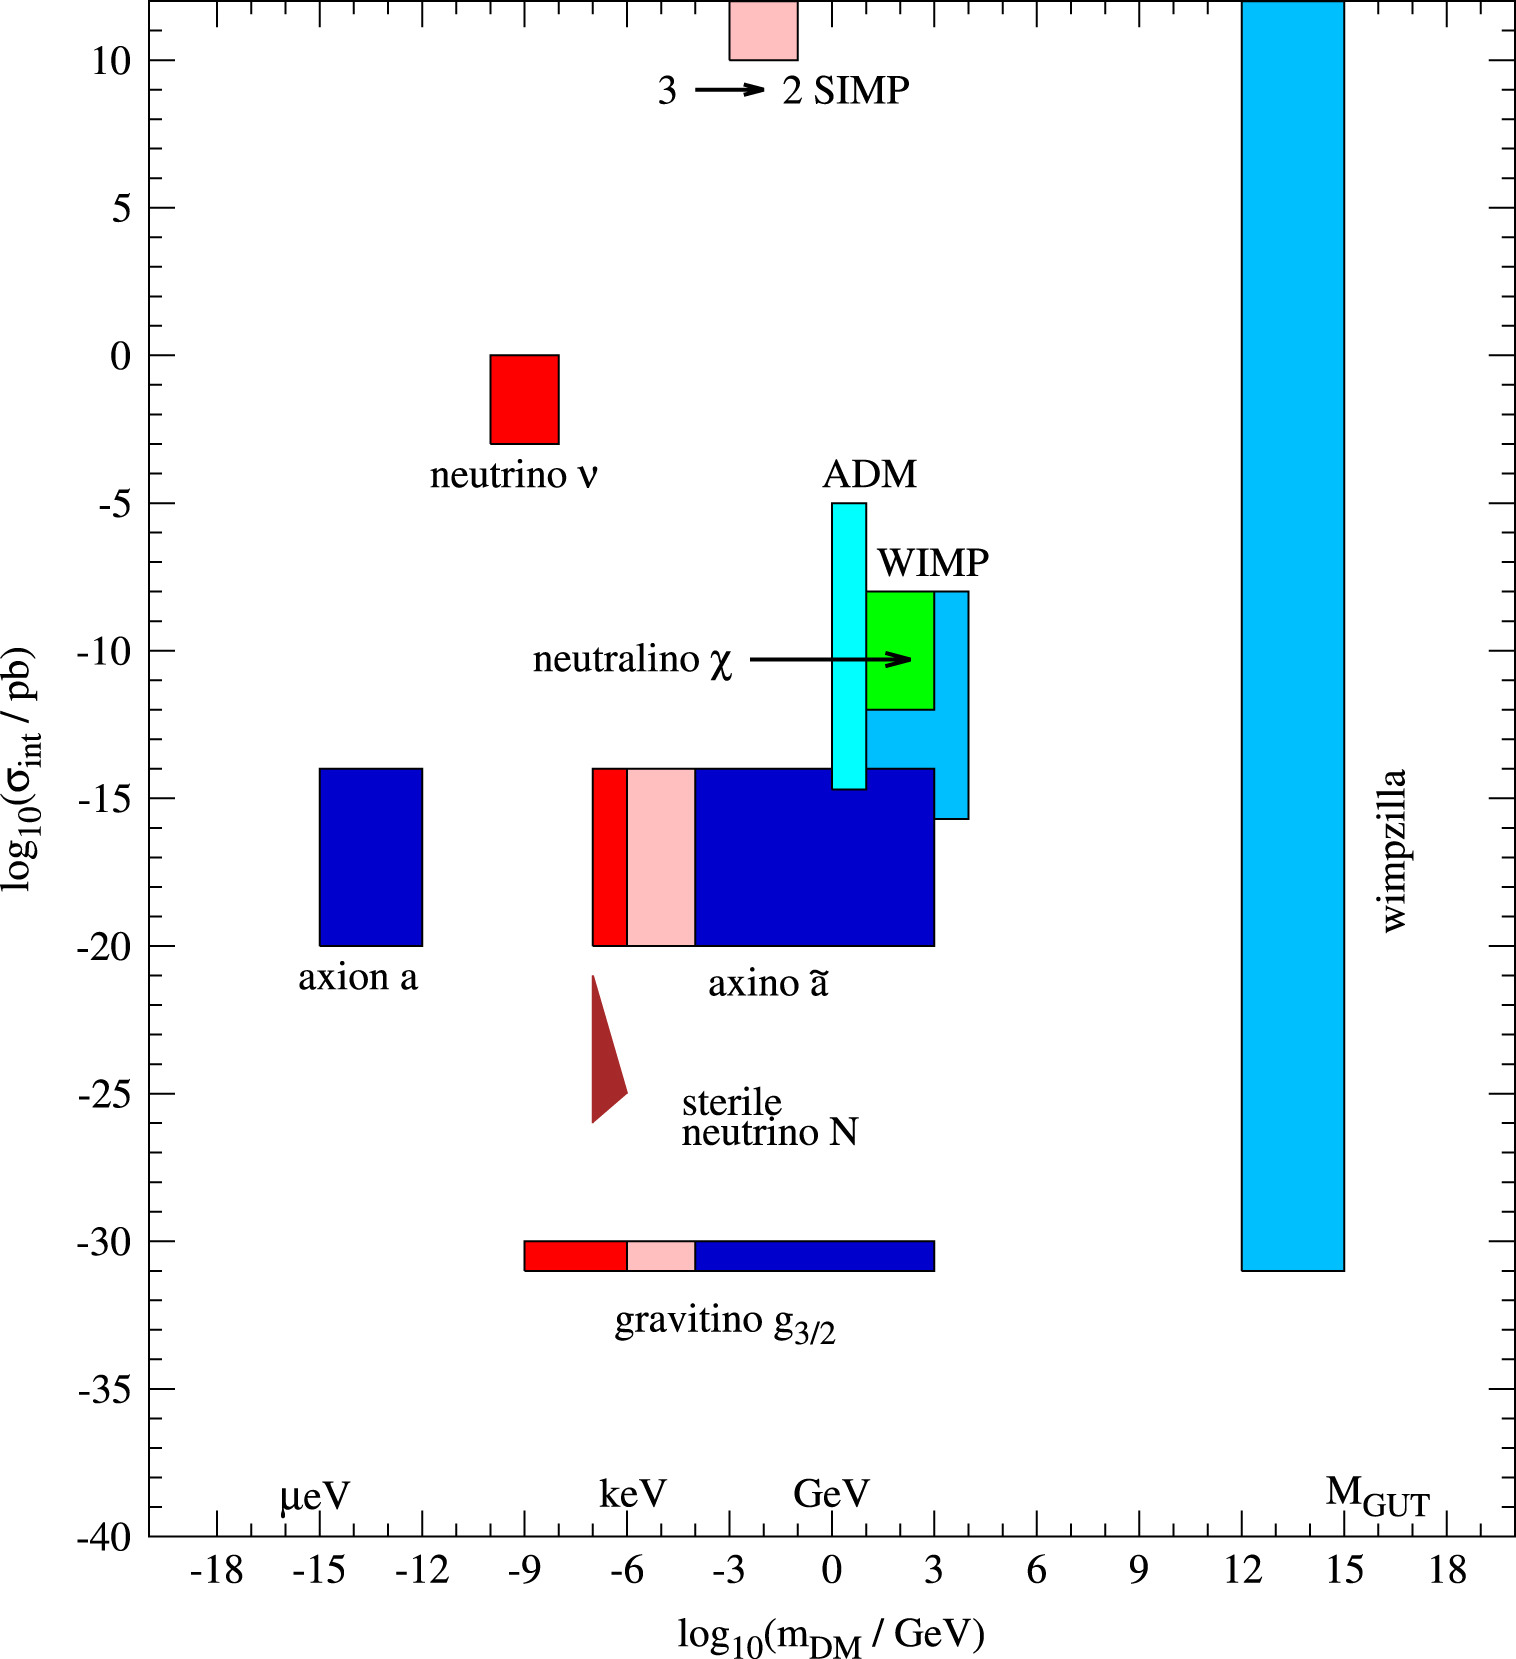
\includegraphics[scale=1]{images/mass_ranges.jpg}
\caption{\cite{BAER20151} Map of the different masses hypthesised for dark matter candidates amongst many theories.}
\label{fig:mass_ranges}
\end{figure}
\par Cosmological findings have been the driving force for dark matter search for the past X years.
The leap to a Weakly Interacting Massive Particle (WIMP) is not a trivial one and must take great care in assumptions
it makes and why it makes them, especially in light of increasing ranges of masses excluded by experiments running today.
The first feature of importance is thus mass.
This is currently under heavy debate in the scientific community as there are supporters of a MILLI mass while on the other spectrum most standard direct
detection experiments today are for ranges running from MASSIVE.
Evidence from phenomena such as gravitational lensing and the constant rotational velocities of stars in galaxies with increasing
distance to their galactic centres suggest a candidate of dark matter halos around these celestial objects.
\\
\par From supersymmetrical neutralinos to superheavy dark matter candidates we are looking at a range from GeV/$c^2$ to several TeV/$c^2$ and even higher in certain theories, see Figure \ref{fig:mass_ranges}.
What many of these theories have in common however is that they all produced these WIMP candidates as a bi-product or as required assumptions
to allow their theories to work.
This then strengthens the theory that such a particle should exist and also what regions of mass, energy and interaction type to look for.
These WIMPs are hypothesised to have been in thermal equilibrium with thermal plasma in the early universe.
As the universe expanded and WIMP annihilation rate was less than the Hubble expansion rate, relic density for dark matter was reached.
This brings us to the cross-sections expected for such WIMPs.
Although this varies from theory to theory, we are expecting orders of the weak interaction scale.
\\
\par This incredibly low interaction rate with regular matter makes it a challenge to detect such WIMPs.
There have been efforts at the Large Hadron Collider to detect missing energies and transverse momenta which could be
explained only through a missing new particle in the mass range of a dark matter candidate.
Although, to date, these efforts have translated into constraints of cross sections and mass the search is still active.
\\
\par Another method of search is through indirect detection by observing celestial objects which have a high mass to luminosity disparity.
These include but are not limited to galactic centres, dwarf galaxies and close galaxy clusters.
This method relies on closely monitoring the particle flux coming from these places waiting for self-interactions or decays into measurable standard model particles to occur.
Searches via these methods are made even harder by the fact that the only biproducts most experiments can reliably measure after accounting
for interstellar magnetic fields, other celestial objects and low background limists are neutrinos and specifi gamma ray energies.
\\
\begin{figure}[H]
\centering
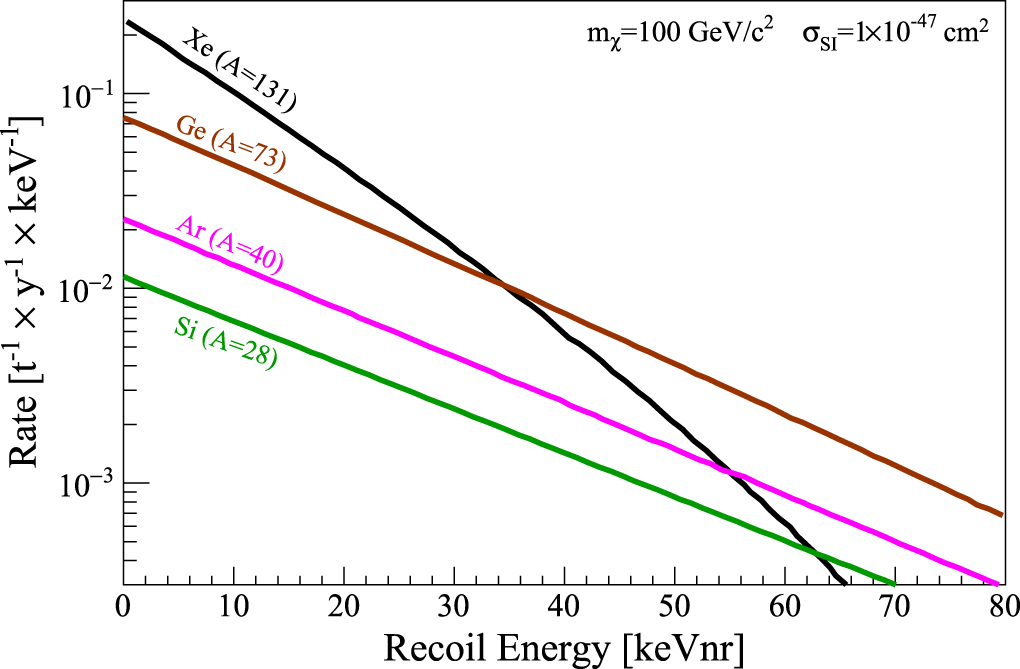
\includegraphics[scale=1]{images/recoil_spectra.jpg}
\caption{\cite{Schumann_2019} Nuclear recoil spctra for varying noble gas targets highlight the better interaction
rate at lower nuclear recoil energies for heavier targets but a lower rate for higher recoil energies.}
\label{fig:recoil_spectra}
\end{figure}
\par Finally, the last method of detection is direct detection.
Large detector chambers are set up, often many kilometers under the earth, essentially waiting for a WIMP
candidate to produce an elastic nuclear recoil with a noble element atom and produce measurable scintillation.
For a WIMP mass ranging between 1 GeV/$c^2$ and 1000 GeV/$c^2$ the recoil energies are in the range 1-100 keV
after which the crossections become way too small for modern detectors.
The choice of noble gas element to use is also non trivial since the rate for spin-indipendent interactions increases with
nucleon number however decreases at high energies due to form factor suppression, as expressed by

often approximated to \cite{lewin1996review}
\begin{equation}
\frac{{\rm{d}}{R}}{{{\rm{d}}{E}}_{\mathrm{nr}}}\propto \exp (- \frac{{E}_{\mathrm{nr}}}{{E}_{0}} \frac{4{m}_{\chi }{m}_{N}}{{({m}_{\chi }+{m}_{N})}^{2}})
\end{equation}
and shown in Figure \ref{fig:recoil_spectra} for increasing mass of the target nucleus.
\\
\par The higher interaction rate for lower recoil energies makes it more probable to detect a WIMP candidate interaction
however these energies produce a lower intensity of scintillation which results in larger errors
 (from sources such as photomultiplier calibration, photon efficiency, dark currents) so there is a compromise to be made.
These interaction rates are directly relatable to our study in teaching an algorithm the photon efficiency maps of the detector
with varying recoil energies.
With the use of Montecarlo simulators such as G4DS one has to incorporate the nuclear recoil spectrum in the simulation setup
and the program will sample from this the Ar40 recoils accordingly.
This process is a long one since this program simulates everything from the interaction to detection.
This process can take several days if running over many energies with all the scintillation being captured.
\\
\par Similarly, our machine learning algorithm is trained uniformally across the different energies but the choice of
dark matter regime to be studied can be changed after training directly through the interaction rate distribution by choosing a suitable nuclear recoil spectrum.
This is where the real advantage presented by this deep learning approach comes into play since the training is done once and changing
sampling distribution can be done virtually instantly and does not require retraining.
\\
\begin{figure}[H]
\centering
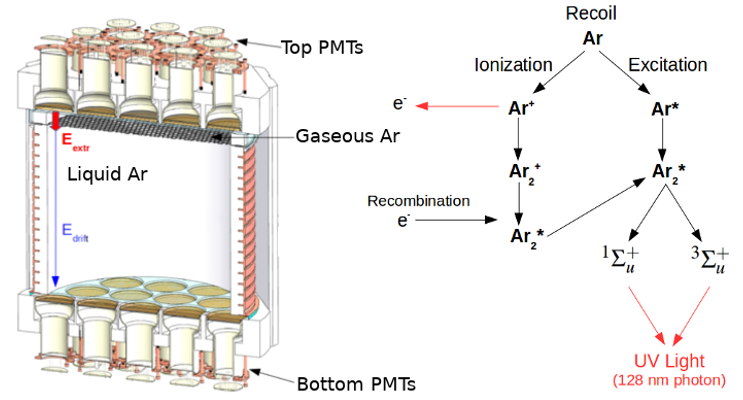
\includegraphics[scale=0.5]{images/detector.png}
\caption{\cite{edkins2017detailed} Schematic of a LAr-TPC and processes of VUV photon emmission.}
\label{fig:detector}
\end{figure}
\par Finally, to understand the variables of interest in this study consider Figure \ref{fig:detector}.
A dark matter particle would enter the detector fiducial volume where it would interact with an Argon nucleus.
The nucleus would then become excited and during de-excitation would emit electrons and produce scintillation.
This first scintillation is known as $S_1$ and has a windows of 7$\mu$s.
After which the electrons would drift upwards due to an electric field within a window of 376$\mu$s.
The electrons would reach a boundary between Argon in the liquid and gaseous phase which would produce a secondary, much more intense scintillation.
Subsequently these photons would be detected by the Silicon PMTs and known as $S_2$ and this window of scintillation is about 30$\mu$s.
The ratio of ionization to scintillation is lower for nuclear recoils than for electron recoils and therefore can be used to place selection cuts to increase sensitivity of the detector.
\\
\par There is a further variable used in the discrimination between background, electron recoils, and nuclear recoil.
This is known as the pulse discrimination shape and relates to the de-excitation modes of the Argon nucleus post-recoil.
As illustrated by Figure \ref{fig:detector} there are two excited states $^{1}\mathrm{{\Sigma_{u}}^{+}}$ and $^{3}\mathrm{{\Sigma_{u}}^{+}}$.
The former has a lifetime of 7ns while the latter has a lifetime of 1600ns.
This difference makes Argon a very competitve candidate as a nuclear target since this same difference in lifetimes between
excited states in Xenon is only about 25ns.
Although Xenon has other benefits and Argon has other sources of background Xenon based TPCs do not have, for LAr-TPC based
detectors this feature is a very good discriminant.
This is due to the fact that the ratio of these excited state lifetimes is related to the stopping power or deposited energy per unit path length
$\frac{dE}{dx}$ and this differs between electron recoils such as gamma photons, alpha particles and
nuclear recoils with argon ion tracks.
Thus a parameter called the Pulse Shape Discriminant denoted by $f$ subscripted by the window of interest of time in ns is used.
We shall use $f_{200}$ defined as
\begin{equation}
f_{200}=\frac{\int_{0}^{200ns}\text{Intensity of photons received}}{\int_{0}^{7\mu s}\text{Intensity of photons received}}.
\end{equation}
Illustrated in Figure \ref{fig:psd} is the simulated difference in Darkside-20k between nuclear and electron recoils for $f_{200}$ against total $S_1$ intensity.
Although normally the parameter $f_{90}$ has been used for experiments such as Darkside-50, for such a much bigger experiment the drift distance is increased substaintially so this
is compensated by using $f_{200}$.
\begin{figure}[H]
\begin{minipage}{.49\textwidth}
  \centering
  \begin{subfigure}{\textwidth}
      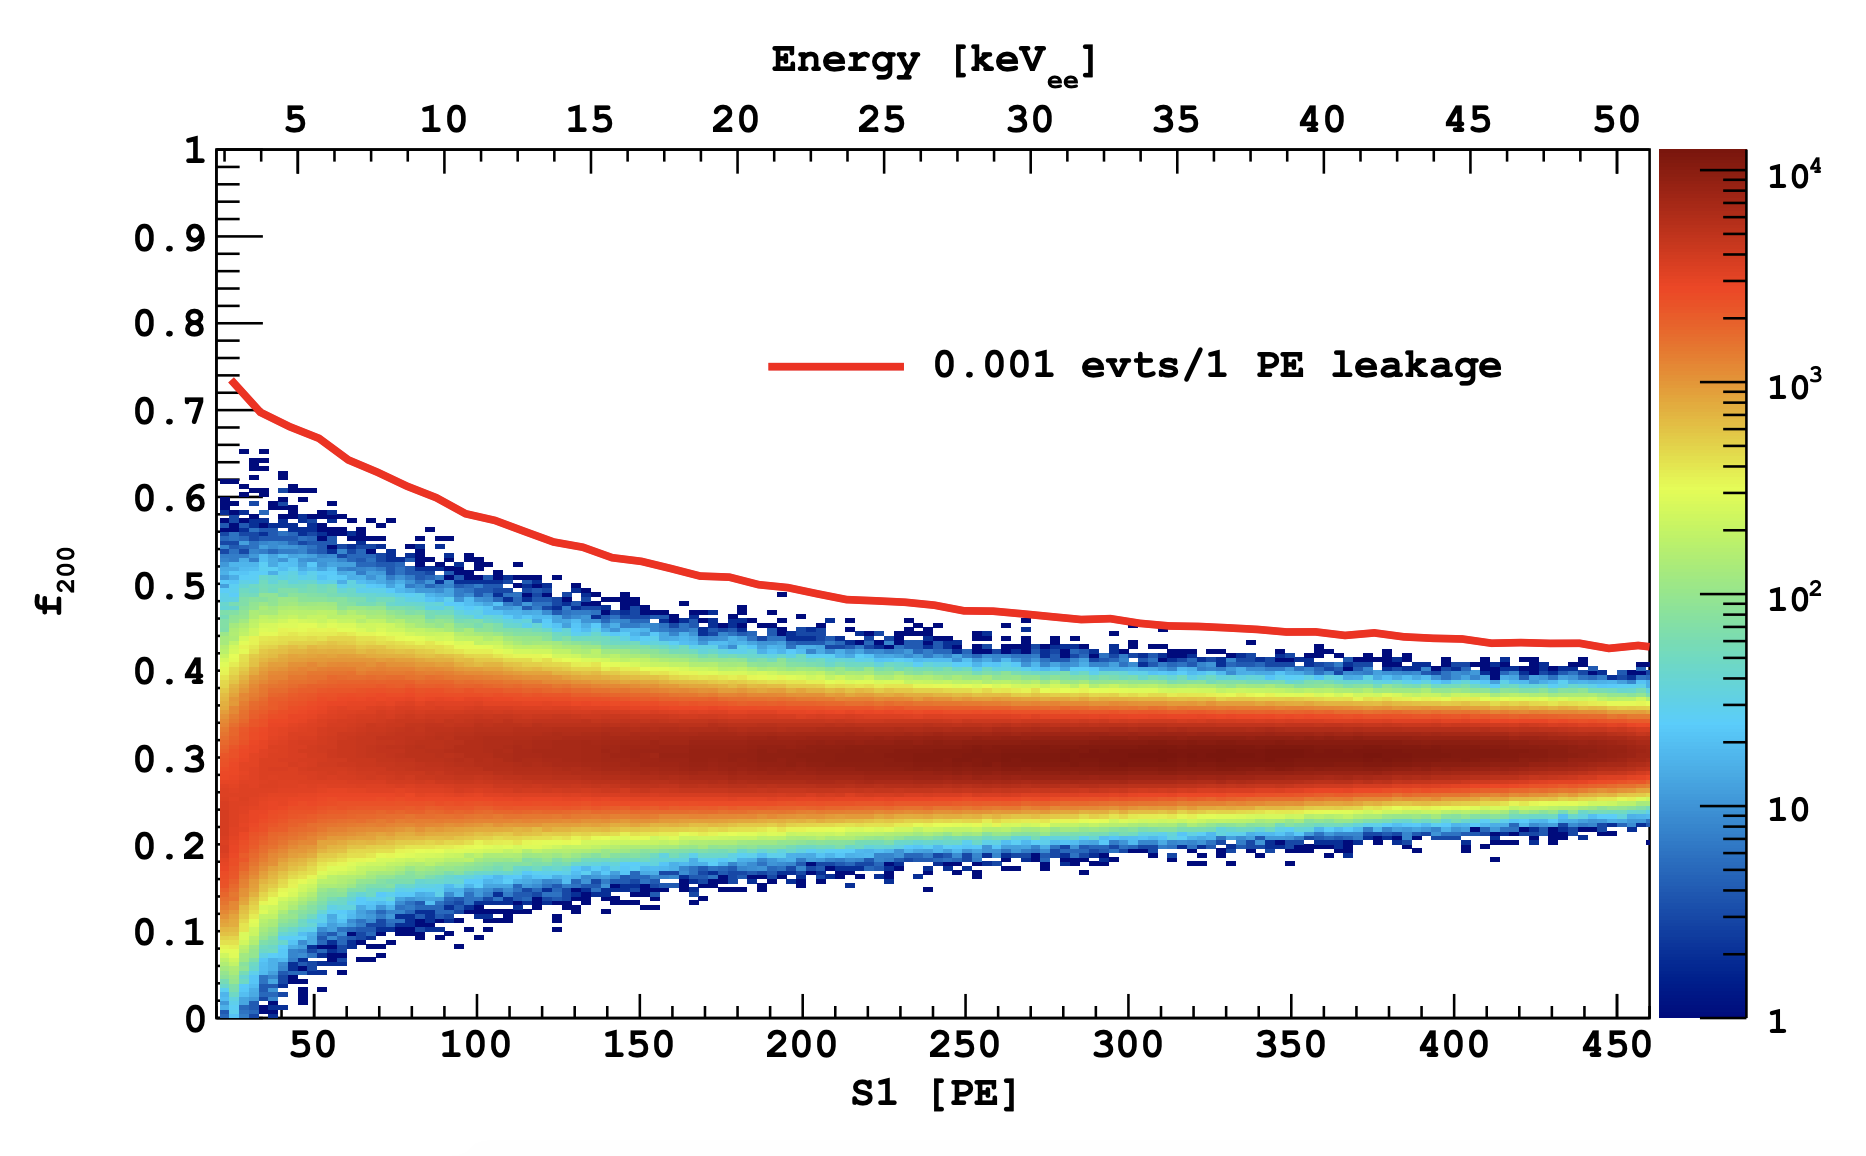
\includegraphics[width=\textwidth]{./images/psd_background.png}
      \subcaption{Simulations for Darkside-20k of $f_{200}$ for background data using $^{39}\mathrm{\text{Ar}}$ $\beta$'s.
      Red line is a leakage curve for a 5-PE requirement on $\beta$'s.}
  \end{subfigure}
\end{minipage}
\begin{minipage}{.49\textwidth}
  \centering
  \begin{subfigure}{\textwidth}
      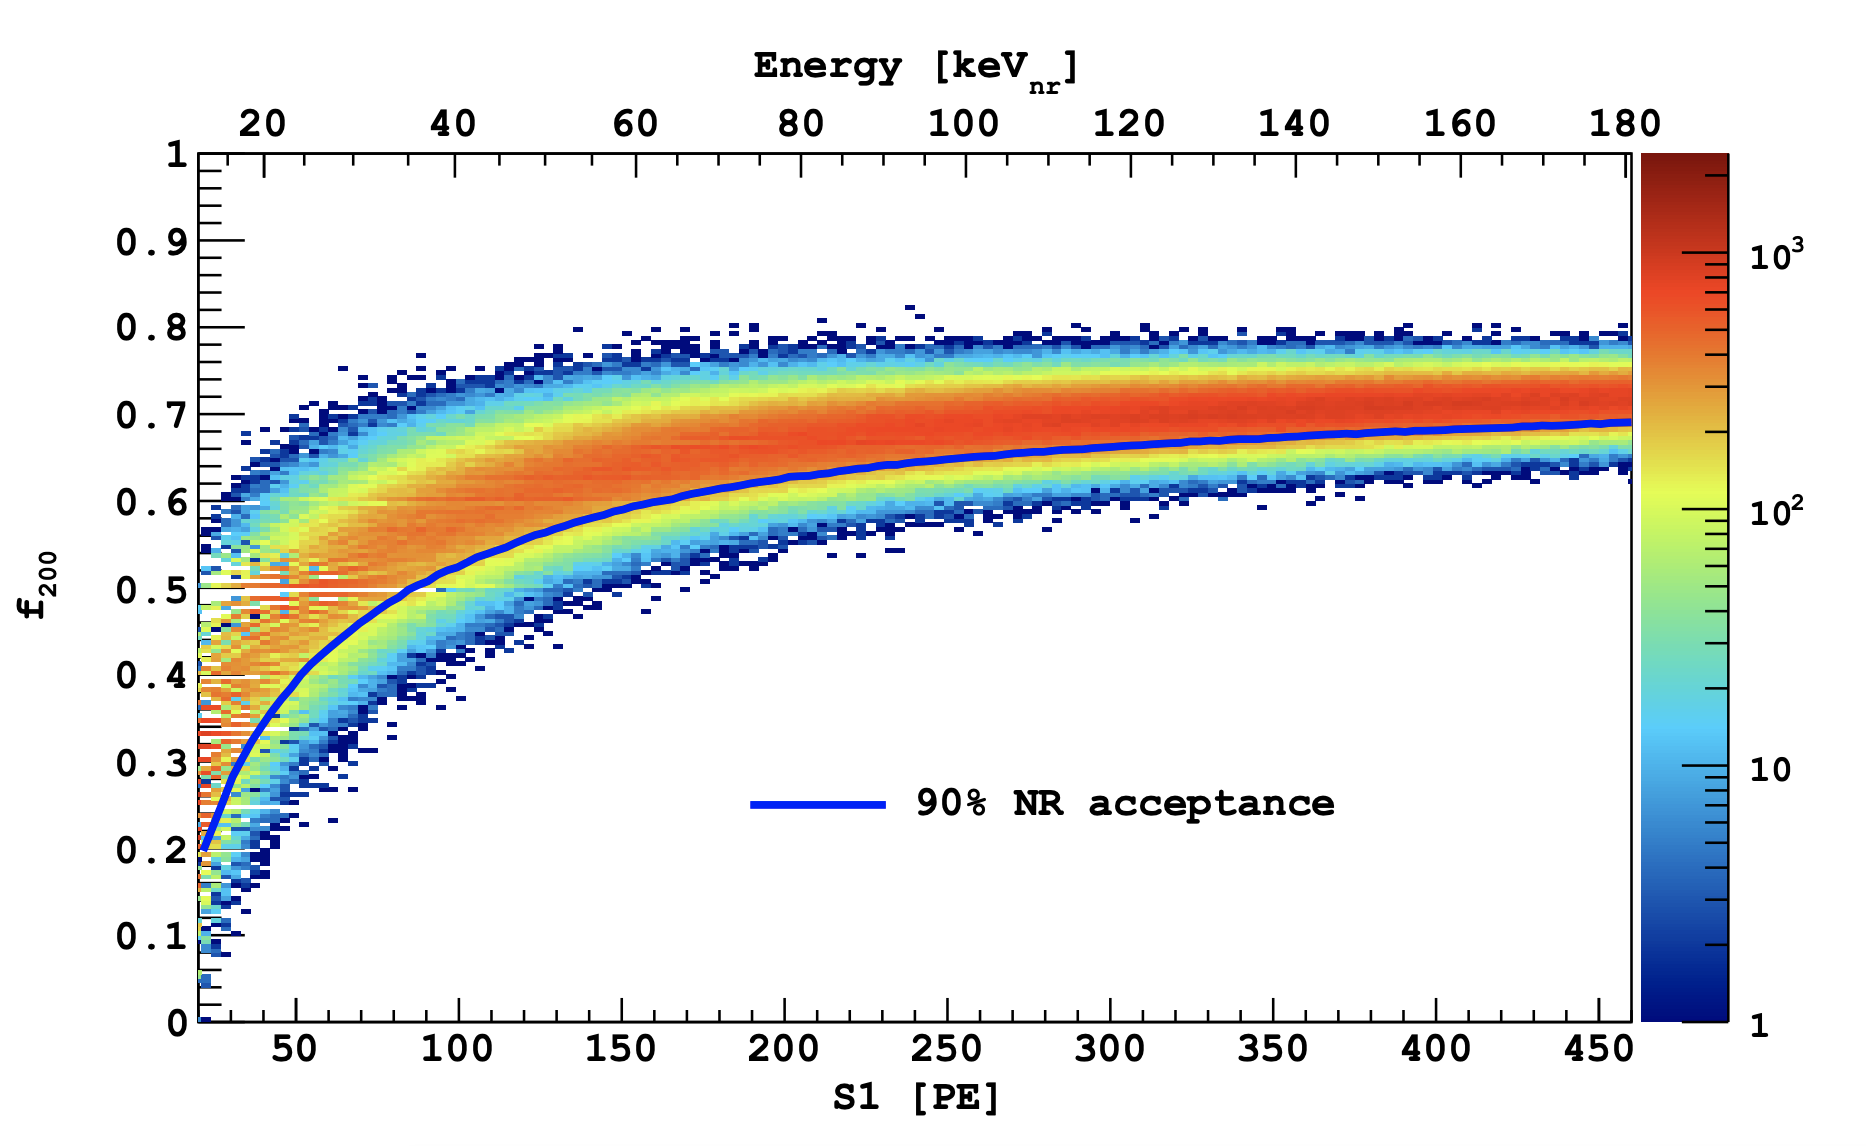
\includegraphics[width=\textwidth]{./images/psd_signal.png}
      \subcaption{Simulations for Darkside-20k of $f_{200}$ for signal nuclear recoils.
      Blue curve is the 90\% NR acceptance region.}
  \end{subfigure}
\end{minipage}
\caption{\cite{aalseth2018darkside} Region of interest using $f_{200}$ pulse shape discriminant against total intensity $S_1$.}
\label{fig:psd}
\end{figure}
\subsection{Current G4DS Results}
The current simulation methods used by the Darkside collaboration consist of very sophisticated and proven Montecarlo methods.
These have been programmed in an opensource program called Geant4 and the complete set of detector macros and routines is called G4DS.
For the purposes of this report and our study we ran G4DS with the following configuration detailed in Table \ref{table:g4ds_config}.
\begin{table}[!h]
\centering
\begin{tabular}{l|l}
\hline
Drift Field & 200V \\
TPC Height & 262cm \\
TPC Width & 150cm \\
Thickness Acrylic Walls & 5cm \\
Thickness LArBuffers & 40cm \\
Thickness Veto Shell & 10cm \\
Thickness TPB & 0.1 mm \\
\hline
\end{tabular}
\caption{Table detailing the major features of the detector setup used in G4DS for the purposes of this study.}
\label{table:g4ds_config}
\end{table}
Although the default configuration was used, no cuts were made on any of the data for the purpose of simply studying the reproducing power of the deep learning technique.
We simulated 1000 uniformly distributed events per $^{40}\mathrm{\text{Ar}}$ recoil in the range 5-235 keV in steps of 1 keV.
An example for 1000, 100 keV nuclear recoil event is shown in Figure \ref{fig:example_vars} for each of the three variables $S_1$, $S_2$ and $f_{200}$.
The data for each variable is similar in shape but the ranges are different and the separation in arithmetic means for the 200 different energies is quite small for $f_{200}$
when compared to $S_1$ and $S_2$.
What this means is that there might be difficulty in training a neural network to produce such $f_{200}$ distributions on condition of the energy, since they are not very distinguishable from each other and do overlap.
\begin{figure}[H]
\begin{minipage}{.5\textwidth}
  \centering
  \begin{subfigure}{.9\textwidth}
      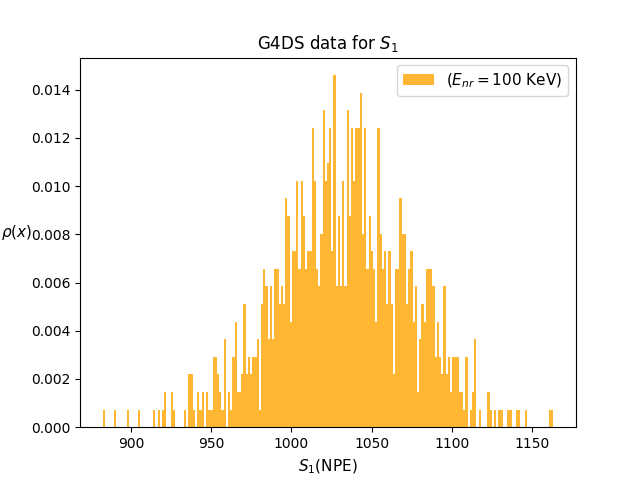
\includegraphics[width=\textwidth]{./images/s1_100.png}
      \subcaption{G4DS generated data for $S_1$}
  \end{subfigure}
\end{minipage}
\begin{minipage}{.5\textwidth}
  \centering
  \begin{subfigure}{.9\textwidth}
      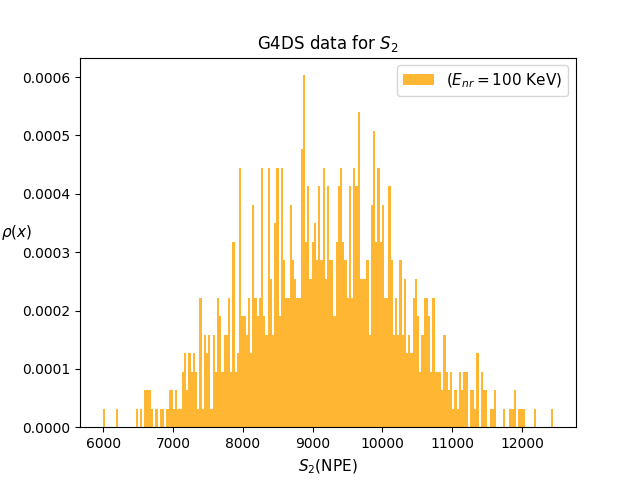
\includegraphics[width=\textwidth]{./images/s2_100.png}
      \subcaption{G4DS generated data for $S_2$}
  \end{subfigure}
\end{minipage}
\end{figure}
\begin{figure}[H]\ContinuedFloat
\centering
\begin{minipage}{.5\textwidth}
  \centering
  \begin{subfigure}{.9\textwidth}
      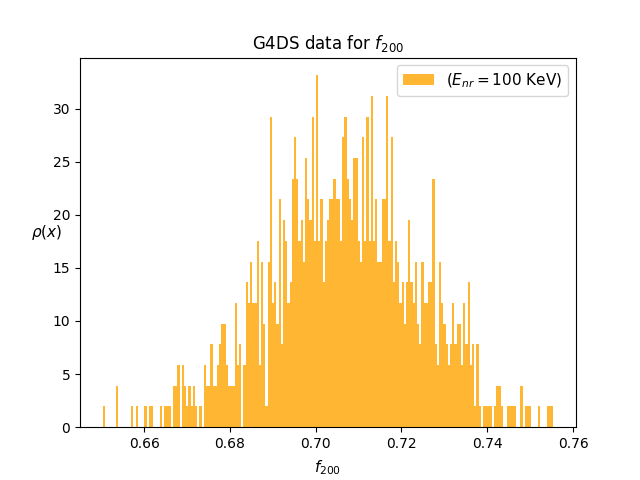
\includegraphics[width=\textwidth]{./images/f200like_100.png}
      \subcaption{G4DS generated data for $f_{200}$}
  \end{subfigure}
\end{minipage}
\caption{Example of the generated data for a run of 1000, 100 keV $^{40}\mathrm{\text{Ar}}$ recoils in G4DS.}
\label{fig:example_vars}
\end{figure}
\par The neural networks described in the next section will therefore be trained on these types of distributions and finally we will want to reproduce
plots such as Figure \ref{fig:psd} to check that the connection between the three variables has been understood to an extent.
To produce a plot for $f_{200}$ vs $S_1$ first a mass for the WIMP is chosen, in this case we take log$(m)=1.5$ which corresponds to a 31.5 GeV/$c^2$ mass.
From theory the corresponding recoil energy spectrum is chosen, shown by Figure \ref{fig:recoil}.
After sampling 1000 energies these are used to sample from 1000 runs of 1000 $^{40}\mathrm{\text{Ar}}$ recoils in G4DS to then produce Figure \ref{fig:g4ds_results}.
These figures (and similarly for log$(m)=$2,2.5,3,4) will be used to compare all our results with the deep learning technique.
\begin{figure}[H]
\centering
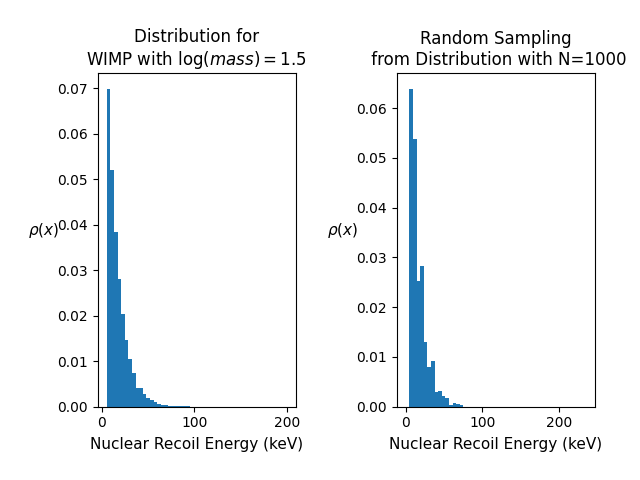
\includegraphics[scale=0.7]{images/Ar_c1dat_m1-5.png}
\caption{A plot of the recoil energy spectrum from theory vs the sampled N=1000 energies spectrum used to work for this mass of WIMP}
\label{fig:recoil}
\end{figure}

\begin{figure}[H]
\begin{minipage}{.5\textwidth}
  \begin{subfigure}{.9\textwidth}
      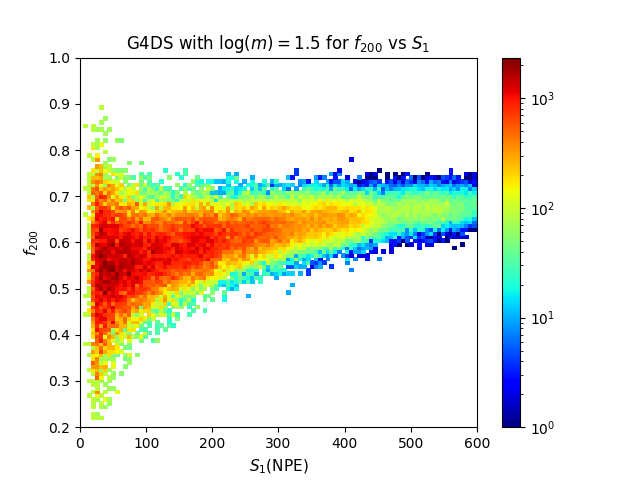
\includegraphics[scale=0.6]{./images/g4_f200_vs_s1.png}
      \subcaption{G4DS generated plotted for $f_{200}$ vs $S_1$ for discrimination, showing events in the signal region.
      As compared with Figure \ref{fig:psd} there is a band of mean value close to $f_{200}=0.7$.}
  \end{subfigure}
\end{minipage}
\begin{minipage}{.5\textwidth}
  \centering
  \begin{subfigure}{.9\textwidth}
      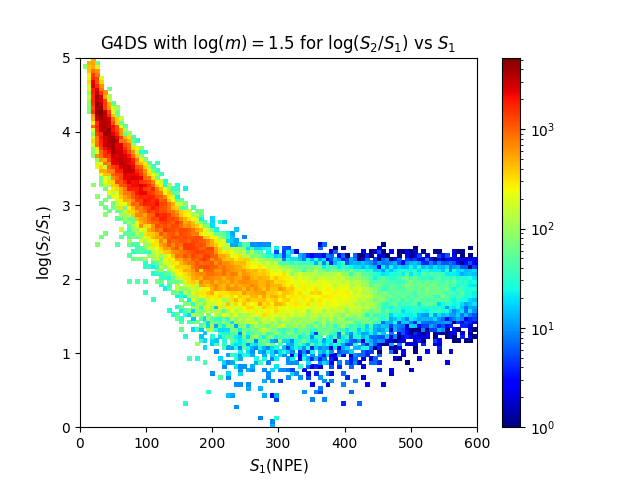
\includegraphics[scale=0.6]{./images/g4_s1_over_s2_vs_s1.png}
      \subcaption{G4DS generated plotted for $S_1$ vs $S_2$ which is another discriminant plot used between signal and background.
      ER would have a smiliar shape but lie above this band of NR with some mixing.}
  \end{subfigure}
\end{minipage}
\caption{Plots commonly used for discriminating between signal and background.
Produced from G4DS data, these plots will be used at the end of our machine learning to compare how well the three variables trained on are understood and their joint probability distributions.}
\label{fig:g4ds_results}
\end{figure}
\subsection{Deep learning as an alternative}
As discussed before, the results obtained with G4DS are well understood and accepted as good simulations (backed up by experiments such as SCENE, DS50).
However, with great detail come large amounts of time waiting for the simulations to complete.
Moreover anytime the nuclear recoil spectrum is changed to simulate different masses of WIMPs, the simulations must be run again.
This hinders progress thatg can be made to an extent since instead of being able to test multiple theories, one must take great care to compromise with time spent waiting.
Lastly, a solution to this could be increasing the number of processors, GPUs and computing capabilities but these cost a lot of money and do not necessarily sale linearly.
It would also be improbable for an institution or a department with a fixed budget it must stick to, to assign more and more resources to one research group which means this is
not a sustainable solution.
\\
\par This is where neural networks appear as a possible solution to this problem.
This will not be a complete overview of machine learning techniques, rather for that please refer to INSERT HERE.
First of all, a neural netowkr is a set of connected nodes in different layers.
Each layer contains many nodes connected to other nodes from successive and previous layers.
Each of these nodes represent intermediary weights to certain functions of output.
In a forward run, the input layers (containing the data to be trained) are connected to
intermediary layers whom carry out some transformation or apply a so called 'activation function' to give
the intermediary weights some values.
This is repeated until the final layer is reached which will usually have an activation function which is dependent on the type of problem at hand.
For example, a classification problem will have weights representing each category which will be largest for the category the algorithm classifies the input as and lower or 0 for the others.
These final weights are then compared to what they should be from the known labelled training data and a quantity to measure 'goodness' of the algorithm is set.
The function doing this is called the loss function.
Acting on this number will be an optimzer which then changes the intermediary weights accoridingly so that ideally on the next run
the new weights and activation functions will guide the algorithm towards a better final weights which will minimze loss and maximise accuracy.
\\
\par This is actually only a subset of machine learning known as supervidsed learning.
The other kind, unsupervised learning, is what we carry out in the algorithms detailed in this report where we essentially want dimensionality reduction.
Particularly, we make use of a rather new method of machine learning known as Generative Adverserial Networks.
In our case we have two neural networks, one known as the classifier and the other as the generator.
The aim of the generator is to reproduce training data as close as possible while the job of the classifier is to
spot at each iteration of training (known as an epoch) which of the two inputs it is being presented by, real or generated.
Their loss functions are connected together by the equation
\\
For the ideal case where the generartor is perfect the accuracy of the discriminator results in around 0.5 as it would have no real clue other than a 50-50 chance to tell the difference.


\section{Methods and Results}
\subsection{Problems in previous work}

\subsection{Novel techniques}

\subsection{Results}
\subsubsection{Variable Learning}

\subsubsection{Analysis and Final Product}


\section{Final Remarks}

\newpage
\printbibliography

\end{document}
